%%%%%%%%%%%%%%%%%%%%%%%%%%%%%%%%%%%%%%%%%
% University/School Laboratory Report
% LaTeX Template
% Version 3.1 (25/3/14)
%
% This template has been downloaded from:
% http://www.LaTeXTemplates.com
%
% Original author:
% Linux and Unix Users Group at Virginia Tech Wiki 
% (https://vtluug.org/wiki/Example_LaTeX_chem_lab_report)
%
% License:
% CC BY-NC-SA 3.0 (http://creativecommons.org/licenses/by-nc-sa/3.0/)
%
%%%%%%%%%%%%%%%%%%%%%%%%%%%%%%%%%%%%%%%%%

\documentclass[paper=letter, fontsize=11pt]{article}

% packages
\usepackage{fixltx2e}
\usepackage[pdftex]{graphicx}
\usepackage{caption, subcaption}
\usepackage{color, wrapfig}

\usepackage{xfrac}
\usepackage{amsmath}  % required for some math elements 
\usepackage{amssymb}

\usepackage{fancyvrb, listings}  % for code verbatim and console outputs
\usepackage[margin=1in]{geometry}

\definecolor{dkgreen}{rgb}{0,0.6,0}
\definecolor{gray}{rgb}{0.5,0.5,0.5}
\definecolor{mauve}{rgb}{0.58,0,0.82}
\definecolor{black}{rgb}{0,0,0}

\lstset{frame=tb,
    language=R,
    aboveskip=3mm,
    belowskip=3mm,
    showstringspaces=false,
    columns=flexible,
    basicstyle={\small\ttfamily},
    numbers=none,
    numberstyle=\tiny\color{gray},
    keywordstyle=\color{blue},
    commentstyle=\color{dkgreen},
    stringstyle=\color{mauve},
    breaklines=true,
    breakatwhitespace=true,
    tabsize=4,
    escapechar={\?}
}

\newcommand{\n}{\newline\newline}

\setlength\parindent{0pt} % removes all indentation from paragraphs

% redefine \VerbatimInput
\RecustomVerbatimCommand{\VerbatimInput}{VerbatimInput}{
    fontsize=\footnotesize,
    frame=lines,  % top and bottom rule only
    framesep=2em,  % separation between frame and text
    rulecolor=\color{black},
    label=\fbox{\color{black}main.R},
    labelposition=topline,
}

%----------------------------------------------------------------------------------------
%	DOCUMENT INFORMATION
%----------------------------------------------------------------------------------------

\title{Project 3 \\ STAT 355}  % Title
\author{Sabbir \textsc{Ahmed}}  % Author name
\date{\today}  % Date for the report

\begin{document}

    \maketitle % Insert the title, author and date

    \section{Part 1}
    \subsection{Question}
    An oceanographer wants to test, on the basis of a random sample of size 35, whether the average depth of the ocean in a certain area is 72.4 fathoms. At the 0.05 level of significance, what will the oceanographer decide if she gets a sample mean of 73.2? Assume the population standard deviation is 2.1.

    \subsection{Answer}
    The null hypothesis, $H_{0}$, claims the mean depth of the ocean in a certain area is 72.4, while the alternative hypothesis, $H_{a}$, says otherwise.

        \[ H_{0}: \mu = 72.4 \ vs \ H_{a}: \mu \neq 72.4 \]

    Since the population mean and standard deviation are known with a sample size of $n > 30$, the Z-score was calculated as follows:

        \begin{equation*}
    Z=\frac{\overline{X}-\mu}{\sfrac{\sigma}{\sqrt{n}}}
    =\frac{73.2-72.4}{\sfrac{2.1}{\sqrt{35}}}=2.2537
    \end{equation*}\newline

    The following snippet was used to generate the Z-test and its probability:
\begin{lstlisting}
    X <- 73.2
    mu <- 72.4
    sigma <- 2.1
    n <- 35
    alpha <- 0.05

    dumpComputation(X=X, mu=mu, sigma=sigma, n=n, 
        alpha=alpha, distType="Z", twoSided=TRUE, "part1")
\end{lstlisting}

    The test statistic was computed to be:

    \begin{equation*}
        Z_{1-\sfrac{0.05}{2}}=Z_{0.975}= 1.96 < 2.2537
    \end{equation*}

    The p-value was computed with the following snippet:
\begin{lstlisting}
    pScore <- 2 * (1 - (pnorm(score)))
    # 0.0242
\end{lstlisting}

    Since $Z_{\sfrac{\alpha}{2}} < Z$ and the p-score was under 0.05, the null hypothesis is rejected.

    \subsection{Output}

    The first sample mean and standard deviation were computed:

    \[ E(\overline{X}) = 1.000, \ \sigma_{\overline{X}} = 0.329 \]

    All the samples were then used to find the sample mean and standard
    deviation. The theoretical values were also computed based on the
    relationships:

    \[ \mu = np \]
    \[ E(\overline{X}) = np \]
    \[ \sigma = np(1-p) \]
    \[ \sigma_{\overline{X}} = \frac{np(1-p)}{\sqrt{n}} \]


    \begin{table}[h]
        \centering
        \begin{tabular*}{200pt}{@{\extracolsep{\fill}} c c c}

        & \textbf{Actual} & \textbf{Theoretical} \\
        \hline
        $\mu$ & 1.500  & 1.500 \\
        E($\overline{X}$) & 1.518 & 1.500 \\
        $\sigma$ & 1.275 & 1.275 \\
        $\sigma$\textsubscript{$\overline{X}$} & 0.292 & 0.329 \\

        \end{tabular*}
    \end{table}

    \subsection{Output}

    The first sample mean and standard deviation were computed:

    \[ E(\overline{X}) = 1.492, \ \sigma_{\overline{X}} = 0.116 \]

    All the samples were then used to find the sample mean and standard
    deviation. The theoretical values were also computed based on the
    relationships:

    \[ \mu = np \]
    \[ E(\overline{X}) = np \]
    \[ \sigma = np(1-p) \]
    \[ \sigma_{\overline{X}} = \frac{np(1-p)}{\sqrt{n}} \]


    \begin{table}[h]
        \centering
        \begin{tabular*}{200pt}{@{\extracolsep{\fill}} c c c}

        & \textbf{Actual} & \textbf{Theoretical} \\
        \hline
        $\mu$ & 1.500  & 1.500 \\
        E($\overline{X}$) & 1.502 & 1.500 \\
        $\sigma$ & 1.275 & 1.275 \\
        $\sigma$\textsubscript{$\overline{X}$} & 0.101 & 0.116 \\

        \end{tabular*}
    \end{table}

    \section{Part 1}
    \subsection{Question}
    An oceanographer wants to test, on the basis of a random sample of size 35, whether the average depth of the ocean in a certain area is 72.4 fathoms. At the 0.05 level of significance, what will the oceanographer decide if she gets a sample mean of 73.2? Assume the population standard deviation is 2.1.

    \subsection{Answer}
    The null hypothesis, $H_{0}$, claims the mean depth of the ocean in a certain area is 72.4, while the alternative hypothesis, $H_{a}$, says otherwise.

        \[ H_{0}: \mu = 72.4 \ vs \ H_{a}: \mu \neq 72.4 \]

    Since the population mean and standard deviation was known with a sample size of $n > 30$, the Z-score was calculated as follows:

        \begin{equation*}
    Z=\frac{\overline{X}-\mu}{\sfrac{\sigma}{\sqrt{n}}}
    =\frac{73.2-72.4}{\sfrac{2.1}{\sqrt{35}}}=2.2537
    \end{equation*}\newline

    The following snippet was used to generate the Z-value and its probability:
\begin{lstlisting}
    X <- 73.2
    mu <- 72.4
    sigma <- 2.1
    n <- 35

    z <- (X - mu)/(sigma/sqrt(n))
    print(z)  # print the Z-score
    print(pnorm(z))  # print the probability
\end{lstlisting}

    The test statistic was computed to be:

    \begin{equation*}
        \pm Z_{0.05}=\pm 1.96 < 2.2537
    \end{equation*}

    The p-value was computed with the following snippet:
\begin{lstlisting}
    pScore <- 2 * (1 - (pnorm(score)))
    # 0.0242
\end{lstlisting}

    Since $Z_{\sfrac{\alpha}{2}} < Z$ and the p-score was under 0.05, the null hypothesis is rejected.

    \section{Part 5}
Example 8.11 was simulated to plot the power curve for one sample \textit{t} testing. Figure \ref{fig:part5} was reproduced below with the following snippet:

\begin{lstlisting}
    sigma <- 0.1  # standard deviation
    alpha <- qnorm(1-0.05)  # P(Z > alpha)
    xSeq <- c(0, 0.2)  # x bounds

    png(
        filename="figures/part5.png", 
        units="in", width=6, height=4, res=200
    )
    ggplot(NULL, aes(x=x, colour=n, fill=n)) +
        stat_function(data=data.frame(x=xSeq, n=factor(5)), 
            fun=function(x) { pnorm(sqrt(5)*x/sigma - alpha) }) +
        stat_function(data=data.frame(x=xSeq, n=factor(10)), 
            fun=function(x) { pnorm(sqrt(10)*x/sigma - alpha) }) +
        stat_function(data=data.frame(x=xSeq, n=factor(15)), 
            fun=function(x) { pnorm(sqrt(15)*x/sigma - alpha) }) + 
        ylab("Power") + xlab("Difference") + labs(colour="Sample Size")
    dev.off()
\end{lstlisting}


    \begin{figure}[ht]
        \begin{center}
            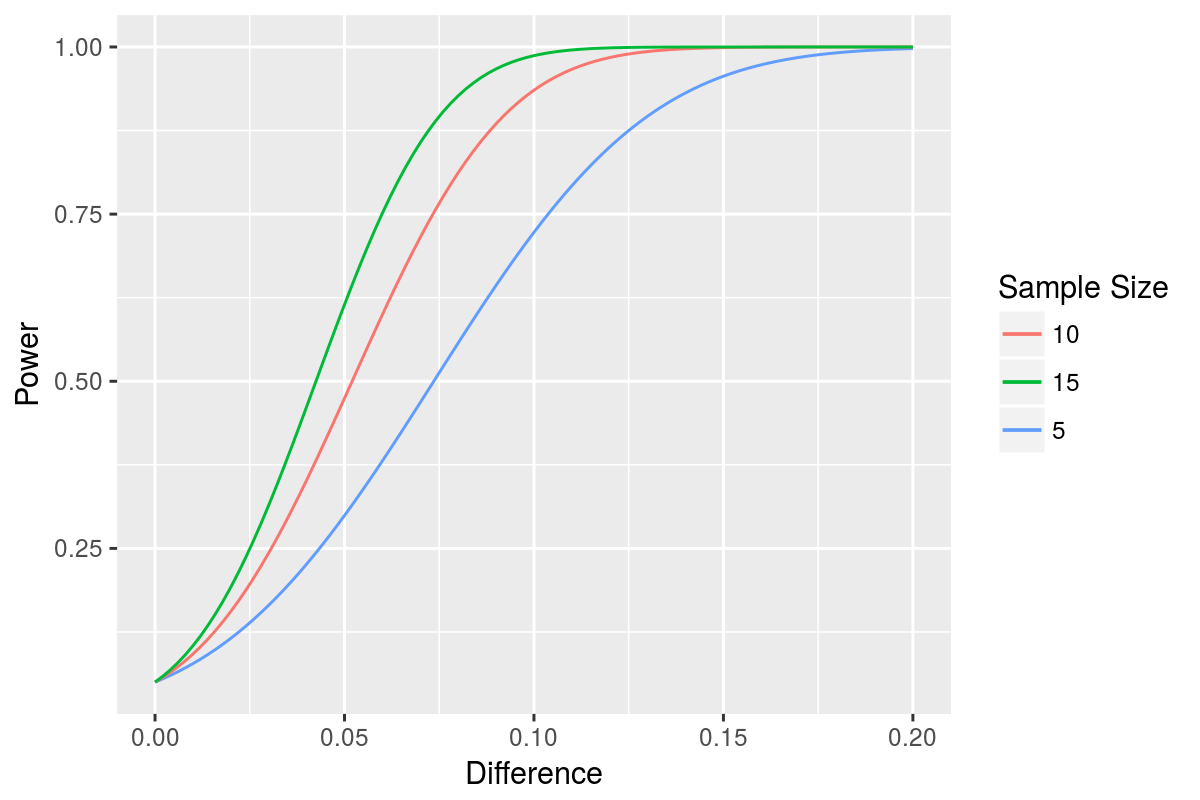
\includegraphics[width=0.7\textwidth]{figures/part5.png}
            \caption{Power Curves for the \textit{t} test Simulated from Example 8.11} \label{fig:part5}
        \end{center}
    \end{figure}

    \section{Part 6}
Example 8.12 was simulated to plot the distribution of the p-values generated from the one sample \textit{t} testing. Figure \ref{fig:part6} was reproduced below with the following snippet:

\begin{lstlisting}
    NUMSAMPS <- 10000

    # initialize distribution variables
    generateHist <- function(mu, filename) {

        # initialize empty arrays
        sampPScores <- generatedData <- rep(0, times=NUMSAMPS)

        # generate 10000 samples
        for (i in 1:NUMSAMPS) {

            generatedData <- rnorm(4, 20, 2)

            # store the sample means in vector
            xbar <- mean(generatedData)
            s <- sd(generatedData)

            tScore <- (xbar - mu)/(s/2)
            sampPScores[i] = pt(tScore, df=3)

        }

        # generate density histograms to display percentage
        h <- hist(
            sampPScores
        )
        h$density = h$counts/sum(h$counts)*100

        # dump plots into PNG
        png(
            filename=paste0("figures/", filename), 
            units="in", width=4, height=4, res=200
        )
        plot(
            h, freq=FALSE,
            main=NULL,
            xlab="P-value",
            ylab="Percent"
        )
        dev.off()

    }

    generateHist(mu=20, filename="part6a.png")
    generateHist(mu=21, filename="part6b.png")
    generateHist(mu=22, filename="part6c.png")
\end{lstlisting}

    \begin{figure}[ht]
        \centering

        \begin{subfigure}[b]{0.5\linewidth}
            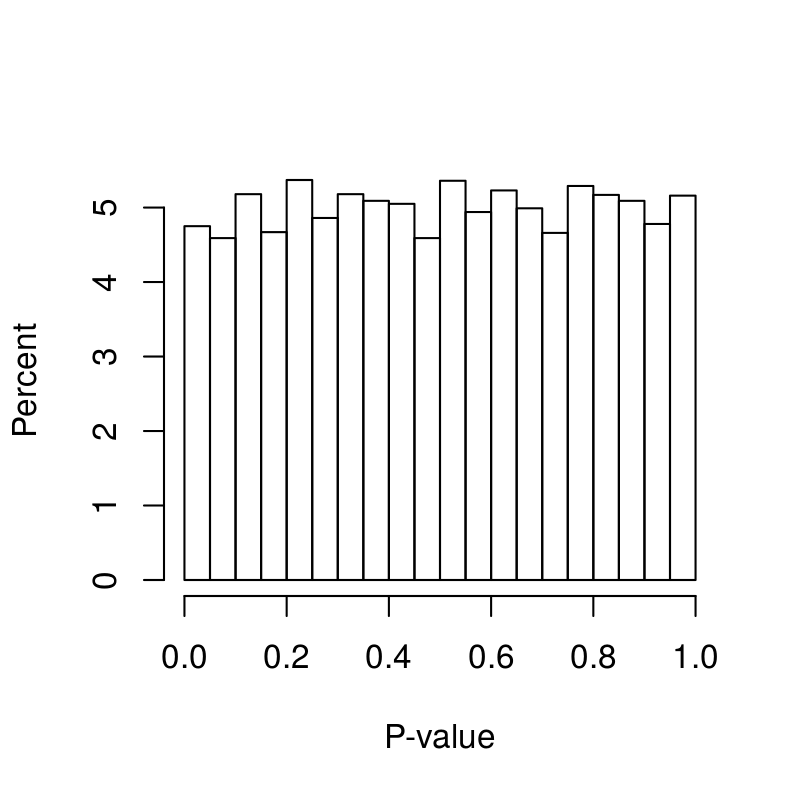
\includegraphics[width=0.9\textwidth]{figures/part6a.png}
            \caption{$\mu=20$}
        \end{subfigure}
        \begin{subfigure}[b]{0.5\linewidth}
            \centering
            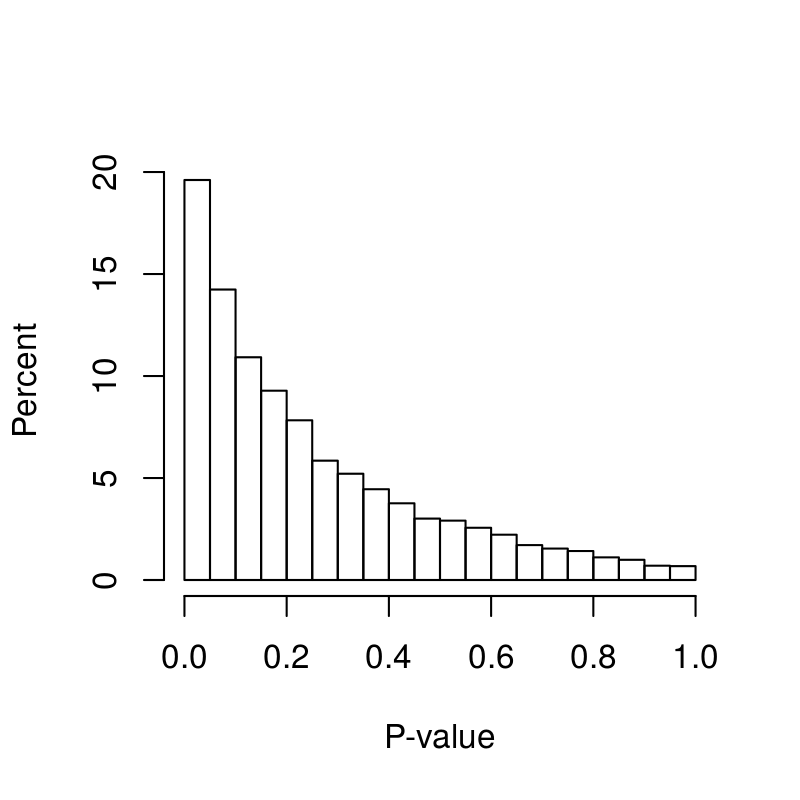
\includegraphics[width=0.9\textwidth]{figures/part6b.png} % first figure itself
            \caption{$\mu=21$}
        \end{subfigure}\hfill
        \begin{subfigure}[b]{0.5\linewidth}
            \centering
            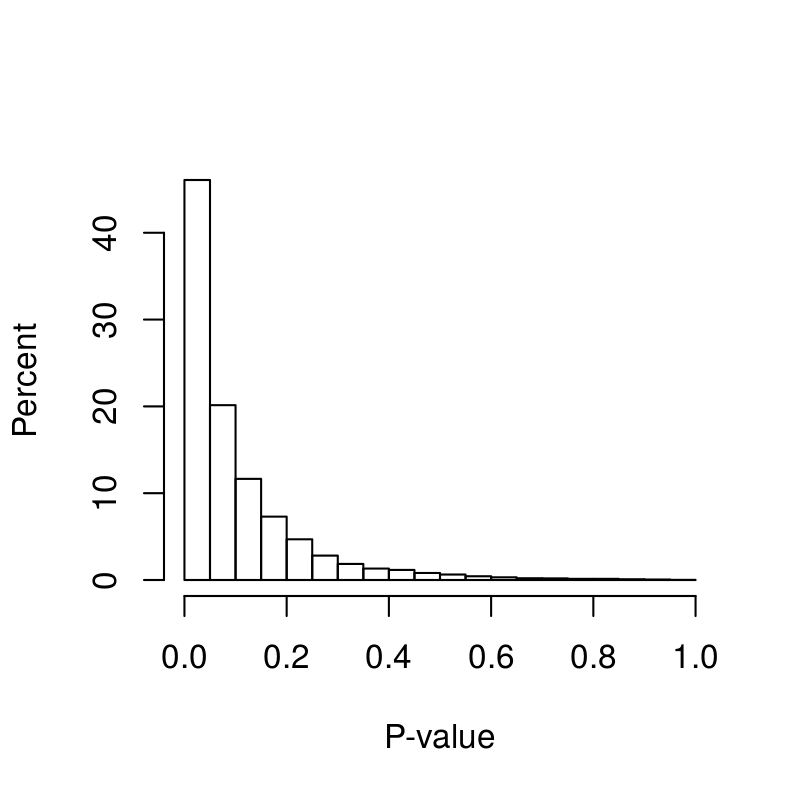
\includegraphics[width=0.9\textwidth]{figures/part6c.png} % second figure itself
            \caption{$\mu=22$}
        \end{subfigure}
        \caption{P-value Simulations for Example 8.12}
    \end{figure} \label{fig:part6}


    \clearpage
    \newpage
    \VerbatimInput{main.R}

\end{document}
